\documentclass[11pt,letterpaper]{article}
% Layout follows the SSAC "Paper Template": 1in sides, 1.1in top, 1.2in bottom,
% Cambria 11pt single spaced with 11pt after each paragraph, 42 Analytics logo bottom left.
\usepackage[left=1in,right=1in,top=1.1in,bottom=1.2in,footskip=0.3in]{geometry}
\usepackage[T1]{fontenc}
\usepackage{caladea}      % metric-compatible free clone of Cambria
\usepackage{amsmath}
\usepackage{amssymb}
\usepackage{booktabs}
\usepackage{float}
\usepackage[section]{placeins}
\usepackage{graphicx}
\graphicspath{{figs/}{./}}
\usepackage{xcolor}
\usepackage{tikz}
\usetikzlibrary{arrows.meta,positioning,fit,calc,shapes.geometric,backgrounds}
\newcommand{\toreview}{\textcolor{red}{\textbf{[TO REVIEW]}}~}
\usepackage[numbers]{natbib}
\setlength{\bibsep}{3pt}
\usepackage{titlesec}
\usepackage{fancyhdr}
\usepackage{eso-pic}
\usepackage{hyperref}
\hypersetup{colorlinks=true,linkcolor=black,citecolor=black,urlcolor=blue}

\setlength{\parindent}{0pt}
\setlength{\parskip}{11pt}
\titleformat{\section}{\fontsize{16}{19}\selectfont\bfseries}{\thesection.}{0.4em}{}
\titleformat{\subsection}{\fontsize{12}{14}\selectfont\bfseries}{\thesubsection.}{0.4em}{}
\titleformat{\paragraph}[runin]{\normalsize\bfseries}{}{0pt}{}
\titlespacing*{\section}{0pt}{6pt}{0pt}
\titlespacing*{\subsection}{0pt}{0pt}{-8pt}
\titlespacing*{\paragraph}{0pt}{0pt}{0.6em}
% after titlesec, which otherwise redefines \subsection and drops the barrier
\let\oldsubsection\subsection
\renewcommand\subsection{\FloatBarrier\oldsubsection}

\pagestyle{fancy}
\fancyhf{}
\renewcommand{\headrulewidth}{0pt}
\cfoot{\thepage}
\AddToShipoutPictureBG{\AtPageLowerLeft{\hspace*{0.9in}\raisebox{0.38in}{
\includegraphics[width=1.95in]{42analytics-logo.png}}}}

\newcommand{\papertitle}{Conditional Queries Against a Learned Hitter Process Model}
\newcommand{\papertrack}{Baseball}  % TODO: confirm track
\newcommand{\paperid}{Paper ID}     % TODO: SSAC paper ID


\begin{document}
\raggedright
\thispagestyle{fancy}
\begin{center}
{\fontsize{18}{22}\selectfont\bfseries \papertitle\par}
\vspace{11pt}
{\fontsize{14}{17}\selectfont \papertrack\par \paperid\par}
\end{center}

% Nate's abstract (paper/abstract.tex): text verbatim, one paragraph in the Alcorn (2018) format.
% Changes: 5 heads -> 6; section headings, Table/Figure pointers and code link dropped (the floats
% moved to 3.2 and 3.3, the link is in 2.2).
\begin{center}{\fontsize{16}{19}\selectfont\bfseries Abstract}\end{center}
\vspace{-11pt}
In baseball, understanding how to use great hitters is often a simple task: play as many of them as you can and play them often. Teams try to gain an edge with the remaining hitters, but less playing time means thinner data in an area that takes hundreds of plate appearances to stabilize. This paper asks whether a model trained on pitches can project how a hitter will do against a type of matchup, like handedness or a specific pitcher, with less data than standard projections need. We train a neural network inspired by (batter$|$pitcher)2vec that learns player embeddings from hitter-controlled pitch outcomes, which decreases the impact of outcome luck. A plate appearance is broken into 6 heads: swing decision, contact, and quality decomposed as exit velocity, launch angle, and spray direction, each conditioned on the pitcher and the game state. The model trains on 6.5 million Statcast pitches from 2015 through 2024 covering 1,672 hitters, each represented as a 64-dimensional embedding. To query it, we reweight which pitchers the projection is drawn over and compose the outputs through the count-state Markov chain into a projected wOBA, so a new split needs a new weight vector, not a retrained model. We test side-specific wOBA against left- and right-handed pitchers on sealed 2025 data against gradient-boosted and empirical Bayes baselines, using RMSE and weighted rank correlation, grouped by prior plate appearances (PA). The model did not pass our pre-registered test. Pooled RMSE was tied (0.0452 against 0.0453 for gradient boosting and 0.0460 for empirical Bayes) and pooled rank correlation was higher (0.47 against 0.42 and 0.40). It beat both baselines on both measures only for hitters with 113 to 451 prior plate appearances, an exploratory result. On 2024, the season used to select the model, it recovers 60\% of the rank-order signal and 64\% of the level signal that one season of data can measure. Without being given definitions of power or contact, the embedding still separates hitters on both, with held-out accuracy of 0.79 and 0.75 against 0.33 by chance, and observed wOBA rises toward high power and high contact. The model is better at ordering hitters within a split than at predicting how many points of wOBA the split is worth. For a team, that makes it most useful for ranking platoon options among hitters with a moderate track record, where the decision is actually in question, not as a replacement for a projection system on raw accuracy.


% =====================================================================================
\section{Introduction}
\label{sec:intro}

% Source: src/analysis/claim1_eval.py STABILIZATION_N_STAR = 226 (variance-components estimate,
% training seasons, hitters only).
Most lineup decisions are simple, because a team's best hitters play every day against every kind of pitcher. The decisions that leave room for an edge involve the bench and platoon hitters, and they usually depend on a split, which is how a hitter performs against one kind of pitcher. Examples include choosing which of two bench hitters starts against a left-handed pitcher and which pinch hitter to send up against the reliever warming up. Bench and platoon hitters are also the ones with the least data. In the training seasons, it takes about 226 plate appearances (PA) against left-handed pitchers before half of the variation in hitters' wOBA against them reflects skill rather than noise (Section~\ref{sec:eval}), and a part-time hitter can take several seasons to reach that many.

Much of that noise enters at the end of the plate appearance. Fielders, parks, and where a ball in play happens to land all change a plate appearance's wOBA value without reflecting anything the hitter did. The hitter's own contribution comes earlier and more often. On each pitch the hitter decides whether to swing, a swing either makes contact or misses, and Statcast records the exit velocity, launch angle, and direction of nearly every ball in play. A plate appearance lasts about four pitches and yields one wOBA value, but it yields several of these pitch-level outcomes, and they carry less of the luck that follows contact.

% Source: alcorn-2018-batter-pitcher2vec.pdf Sections 2.1, 2.2, 4; tango-2009 platoon constants note
% (The Book p.157).
The usual way to project a split is to regress the observed split toward the league split for the hitter's batting side. In \citet[p.~157]{tango2007}, a right-handed hitter needs about 2,200 PA against left-handed pitchers before the observed split receives half the weight, and a left-handed hitter needs about 1,000. As a result, the estimate for most hitters stays close to the league-average split, and two part-time hitters from the same side receive nearly the same projection. This empirical Bayes shrinkage \citep{efron1972} uses only a hitter's outcomes in the split being projected, and it is one of the two baselines in this paper. The other adds summaries of the hitter's own pitches, such as swing, whiff, and exit velocity rates by pitcher hand, in gradient-boosted trees \citep{chen2016}. It uses pitch data only as season rates and does not see individual pitches or the pitchers who threw them.

\citet{alcorn2018} showed that a neural network can learn useful representations of players from their matchups alone. The (batter$|$pitcher)2vec model gave each batter and pitcher a nine-dimension embedding, trained to predict the outcome of each at-bat from the identities of the two players in Retrosheet data from 2013 through 2015. The embeddings grouped similar hitters without being told what made them similar, and they predicted outcome distributions for matchups absent from training better than simpler baselines. Alcorn suggested that predicting PITCHf/x measurements instead of discrete outcomes could convey more about players, and the model in this paper follows that suggestion with Statcast. Each hitter keeps a learned embedding, but the network predicts the hitter's response to each pitch from the pitch's measured characteristics, rather than the at-bat result from the pitcher's identity.

This paper introduces a pitch-level hitter embedding model and a query that turns it into a projected wOBA against any chosen set of pitchers. The model learns from every pitch a hitter has seen and shares structure across hitters through the embedding. A projection is a weighted average over pitchers, so a new split requires a new set of pitcher weights rather than a retrained model. The model was built mainly for hitters with little history against a pitcher hand, but it is meant to be accurate for every hitter. The query is tested on 2025 handedness splits against empirical Bayes and gradient-boosted baselines, and the embedding is examined for what it learned from per-pitch outcomes alone.

% =====================================================================================
\section{Methods}
\label{sec:methods}

\subsection{Data}
\label{sec:data}

% Source: data/processed/phase_d5_clean_final/manifest.json; src/config/split_config*.json;
% decision log 2026-08-01, 2026-09-20.
Pitch-level Statcast data from the 2015 through 2025 regular seasons were used. Each pitch carries its velocity, movement, release point, spin, plate location, pitch type, the count, and the handedness of both players, and each ball in play carries its exit velocity, launch angle, and a spray angle computed from where it was fielded. Pitchouts, automatic balls and strikes, bunts, pitches thrown by position players, pitches to pitchers batting, and pitches missing a core measurement were removed. The final data set consisted of 7,245,923 pitches. No minimum exposure was imposed, so every hitter in the training seasons has an embedding.

Model configurations were compared by training on 2015 through 2023 and scoring on 2024, the selection season. The chosen configuration was then retrained on 2015 through 2024, 6,540,616 pitches covering 1,672 hitters and 2,182 pitchers, and evaluated on 2025. Feature scaling was fit on 2015 through 2023 only, and the baselines saw only seasons before the one being scored.

\subsection{Model}
\label{sec:model}

% Source: paper/draft3/fig_arch.tex
\begin{figure}[!ht]
\centering
% fig_arch.tex -- architecture (a) and query (b) schematic. \input inside a figure env.
% needs: tikz with arrows.meta, positioning, fit, calc, shapes.geometric, backgrounds; amsmath; xcolor
\begin{tikzpicture}[
  x=1cm, y=1cm, font=\scriptsize, text=black!80, line width=0.5pt,
  box/.style={draw=black!55, rounded corners=1.5pt, align=center, inner sep=2pt,
              minimum height=0.5cm},
  acc/.style={draw=blue!60, fill=blue!7},
  bar/.style={draw=black!55, fill=black!5, rounded corners=1.5pt,
              minimum width=0.46cm, minimum height=5.6cm},
  head/.style={box, minimum width=3.2cm, anchor=west},
  arr/.style={-{Stealth[length=3.5pt,width=3pt]}, draw=black!60},
  cond/.style={-{Stealth[length=3pt,width=2.6pt]}, draw=blue!60, densely dashed},
  ttl/.style={anchor=west, font=\footnotesize\bfseries},
  note/.style={text=black!60},
  cnt/.style={draw=black!45, rounded corners=1pt, inner sep=0pt, minimum width=0.42cm,
              minimum height=0.26cm, font=\tiny},
  stepc/.style={circle, draw=blue!60, fill=blue!7, inner sep=0pt, minimum size=0.38cm,
                font=\scriptsize\bfseries},
  para/.style={anchor=north west, align=left, inner sep=0pt},
]

% ---------------------------------------------------------------- (a) the network
\node[ttl] at (0,8.55) {(a) The network};

\node[box, acc, minimum width=2.45cm] (hid) at (1.25,7.55) {Hitter ID $h$};
\node[box, acc, minimum width=2.45cm] (emb) at (1.25,6.65) {Embedding (64)};
\node[box, minimum width=2.45cm, text width=2.3cm] (ctx) at (1.25,4.9)
  {Pitch context (46)\\[1pt]{\tiny\color{black!60}physical measurements,
   location, type, handedness of both players, count}};
\node[box, minimum width=2.45cm] (c1) at (1.25,3.45) {Context layer (128)};
\node[box, minimum width=2.45cm] (c2) at (1.25,2.55) {Context layer (128)};
\draw[arr] (hid) -- (emb);
\draw[arr] (ctx) -- (c1);
\draw[arr] (c1) -- (c2);

\node[bar] (cat) at (3.05,5.0) {};
\node[bar] (t1)  at (3.8,5.0)  {};
\node[bar] (t2)  at (4.55,5.0) {};
\node[rotate=90] at (cat) {Concatenate (64 + 128)};
\node[rotate=90] at (t1)  {Trunk layer (256)};
\node[rotate=90] at (t2)  {Trunk layer (256)};
\draw[arr] (emb.east) -- (cat.west |- emb.east);
\draw[arr] (c2.east)  -- (cat.west |- c2.east);
\draw[arr] (cat) -- (t1);
\draw[arr] (t1) -- (t2);

% six heads, top to bottom in plate-appearance order
\foreach \name/\y/\lbl in {
    sw/7.45/{Swing},
    co/6.47/{Contact $\mid$ swing},
    sp/5.49/{Foul/tip/in play $\mid$ contact},
    ev/4.51/{Exit velocity {\color{black!60}(24 bins)}},
    la/3.53/{Launch angle $\mid$ EV {\color{black!60}(24)}},
    sy/2.55/{Spray $\mid$ EV, LA {\color{black!60}(24)}}} {
  \node[head] (\name) at (5.1,\y) {\lbl};
  \draw[arr] (t2.east |- \name.west) -- (\name.west);
}
% EV and LA bins feed the later heads
\draw[cond] (ev.east) to[out=0, in=0, looseness=1.3] (la.east);
\draw[cond] (ev.east) to[out=0, in=0, looseness=1.1] (sy.east);
\draw[cond] (la.east) to[out=0, in=0, looseness=1.3] (sy.east);

\node[box, dashed, draw=black!50, text width=8.1cm, inner sep=3pt] (take) at (4.25,1.3)
  {Take table, fit separately and not part of the network\\[1pt]
   $p(\text{ball},\ \text{called strike},\ \text{HBP} \mid
     \text{location, batter hand, pitcher hand})$};

% panel divider
\draw[black!20] (8.85,0.8) -- (8.85,8.7);

% ---------------------------------------------------------------- (b) a query
\begin{scope}[xshift=9.15cm]
\node[ttl] at (0,8.55) {(b) A query};

% step 1
\node[stepc] (s1) at (0.2,7.9) {1};
\node[para, text width=6.4cm] at (0.55,8.03)
  {For pitcher $j$ and each count, sample 6 of the pitcher's real pitches in that count
   to same-side hitters. Run the network for hitter $h$ and average.\\[3pt]
   {\color{blue!60}$\Rightarrow$} per count $p_B$, $p_S$, $p_F$, $p_H$ and $v(b,s)$,
   the expected wOBA from a ball in play\\(its chance times its average value)};

% step 2, the 12-count chain
\node[stepc] (s2) at (0.2,5.5) {2};
\begin{scope}[shift={(0.95,5.5)}]
  \foreach \b in {0,...,3} \foreach \s in {0,1,2}
    \node[cnt] (n\b\s) at (0.62*\b,-0.48*\s) {\b-\s};
  \foreach \b in {0,1,2} \foreach \s in {0,1,2} {
    \pgfmathtruncatemacro{\nb}{\b+1}
    \draw[arr, draw=black!40] (n\b\s) -- (n\nb\s);}
  \foreach \b in {0,...,3} \foreach \s in {0,1} {
    \pgfmathtruncatemacro{\ns}{\s+1}
    \draw[arr, draw=black!40] (n\b\s) -- (n\b\ns);}
  \node[cnt, acc] at (n00) {0-0};
  \node[note, font=\tiny, anchor=south] at ($(n10.north)!0.5!(n20.north)+(0,0.03)$)
    {balls $\rightarrow$};
  \node[note, font=\tiny, anchor=north] at (n12.south |- 0,-1.15) {strikes $\downarrow$};
\end{scope}
\node[para, text width=3.45cm] at (3.3,5.63)
  {Count-state Markov chain over the 12 counts, solved backward from the end states\\[3pt]
   {\color{blue!60}$\Rightarrow$} $W_{hj} = W(0,0)$};

% step 3
\node[stepc] (s3) at (0.2,3.45) {3};
\node[para, text width=6.4cm] at (0.55,3.58)
  {Weighted mean over the pitcher set $S$, with weights proportional to batters faced};
\node[anchor=west] at (0.5,2.42)
  {$\widehat{\text{wOBA}}_S(h)=\sum_j w^S_j\, W_{hj}, \qquad
    w^S_j\propto \text{BF}_j\,\mathbf{1}[j\in S]$};
\node[box, draw=blue!60, text width=6.2cm, inner sep=3pt, anchor=north west]
  at (0.55,1.98) {A new split is a new set $S$, so only the weights change.
                 No retraining.};

\draw[arr] (s1) -- (s2);
\draw[arr] (s2) -- (s3);
\end{scope}
\end{tikzpicture}

\caption{\toreview (a) The network. A hitter's embedding and the pitch context feed a shared trunk, and six heads predict the hitter-controlled outcomes of the pitch in the order they occur. Taken pitches are read from a separate table. (b) A query. Per-count outcomes against one pitcher are composed through the count into $W_{hj}$, and a weighted average over the chosen pitchers gives the projection.}
\label{fig:arch}
\end{figure}

% Source: src/model/v1.py heads; data manifest n_quality_bins 24; decision log 2026-08-08.
The model architecture can be seen in Figure~\ref{fig:arch}a. Each hitter has a 64-dimension embedding, a learned vector that is the only input identifying the hitter. The same embedding covers all training seasons, and a projection describes the hitter across those seasons together. Each pitch is described by a 46-dimension context vector built from its physical measurements, location, type, the handedness of both players, and the count. The pitcher enters only through the pitches thrown, not through an identifier, which lets the model describe any pitcher whose pitches it has seen. Because the count is the only game state included, predictions reflect the hitter and the pitch rather than the game situation.

The context passes through two layers of 128 units and is then joined with the hitter's embedding in a shared trunk of two layers of 256 units. Six heads read the trunk in the order a plate appearance unfolds. The first three give the probability of a swing, the probability of contact given a swing, and whether contact is a foul, a foul tip, or a ball in play (a two-strike foul tip is a strikeout and a foul is not). The other three give the exit velocity, launch angle, and spray direction of a ball in play, each in 24 bins. Launch angle is predicted given exit velocity, and spray given both, so the three are never treated as independent.

Taken pitches depend mostly on the pitcher and the umpire. Their outcomes therefore come from a table fit on the training seasons, which gives the probability of a ball, a called strike, or a hit batter for each plate location and pairing of batter and pitcher hand.

% Source: src/model/v1.py loss; src/model/train.py masks.
The network is trained to maximize the summed log-likelihood of each hitter's outcomes,
\begin{equation}
\begin{split}
\mathcal{L} = \sum_{i} \Big[ & \log p(a_i) + m^{c}_i \log p(c_i) + m^{t}_i \log p(t_i \mid c_i) + m^{e}_i \log p(e_i) \\
& + m^{l}_i \log p(l_i \mid e_i) + m^{s}_i \log p(s_i \mid e_i, l_i) \Big],
\end{split}
\label{eq:loss}
\end{equation}
where for pitch $i$, $a_i$ is the swing decision, $c_i$ the contact outcome, $t_i$ the contact type (foul, foul tip, or ball in play), and $e_i$, $l_i$, and $s_i$ the exit velocity, launch angle, and spray bins. Every probability is conditioned on the hitter $h$ and the pitch context $x_i$. Each mask $m_i$ is one when the outcome exists and was measured, so contact is scored only on swings, contact type only on contact, and the three quality terms only on measured balls in play.

% Source: results/model_v1/sweep_log.csv stage clean (dim64 five-seed mean 1.023268 vs dim32 1.02378);
% decision log 2026-09-02/03 (SGD table, lr 1.0); checkpoint clean_dim64_final_s0.pt (266,317 parameters).
The network has 266,317 parameters. Weights outside the embedding table are trained with AdamW \citep{loshchilov2019} at a learning rate of $10^{-3}$ and batches of 8,192 pitches. The embedding table is trained with plain stochastic gradient descent at a learning rate of 1.0, because an adaptive optimizer would give a rarely seen hitter steps as large as a regular's, while plain gradient descent moves each embedding in proportion to the hitter's data. Embedding sizes of 32 and 64 were compared, and 64 was chosen because it gave the lower 2024 log loss averaged over five seeds.\footnote{The mean log loss was 1.02327 for 64 dimensions against 1.02378 for 32.} Weight decay of $10^{-2}$ applies to all weights and dropout of 0.1 to the trunk.

Five copies are trained from different seeds as a deep ensemble \citep{lakshminarayanan2017}, and each head's predicted distribution is averaged across the five for the point projection. The model was implemented in PyTorch, and each copy trains on a CPU in about 25 minutes. The code is available at \url{https://github.com/nseluga/hitter-embedding}.

\subsection{Querying the model}
\label{sec:query}

% Source: src/model/query.py docstring; src/model/query_tables.py; decision log 2026-08-08.
The network describes a single pitch, while a lineup decision concerns many plate appearances against many pitchers. A query takes a hitter, a set of pitchers, and a weight for each pitcher, and returns the hitter's projected wOBA per plate appearance against those pitchers. It connects the single pitch to the decision in three steps (Figure~\ref{fig:arch}b).

The first step fixes one pitcher. For pitcher $j$ and each count, the network is run for hitter $h$ on six real pitches that pitcher $j$ threw in that count during the training seasons to hitters who bat from the same side as $h$, and the six outputs are averaged.\footnote{Sparse counts fall back to pitches with the same number of strikes, then to all of that pitcher's pitches to that side. Balls in play that Statcast did not measure, about 7\%, take the league's average value for such balls.} This gives, for each count, the probability that the pitch ends as a ball, a strike, a foul, a hit batter, or a ball in play. The expected wOBA from a ball in play is that probability times the ball in play's average value. The average value adds up the league's average wOBA for every combination of exit velocity, launch angle, and spray bins, each weighted by the hitter's predicted probability of that combination. Each ball in play is thus valued by the league's average result for its bins, not by its actual result. This sets aside the fielder and park effects described in Section~\ref{sec:intro}.

The second step plays out the plate appearance. Each pitch moves the count to a new state or ends the plate appearance, so the expected wOBA from any count is a sum over the possible pitch outcomes. Each term is the probability of that outcome times the expected wOBA of the count or result it leads to. The count moves as a Markov chain over 12 states from 0-0 to 3-2, and the expected wOBA from count $(b,s)$ satisfies
\begin{equation}
W(b,s) = p_B\, W(b+1,s) + p_S\, W(b,s+1) + p_F\, W(b,\min(s+1,2)) + p_H\, w_{\text{HBP}} + v(b,s),
\label{eq:chain}
\end{equation}
where $p_B$, $p_S$, $p_F$, and $p_H$ are the probabilities of a ball, a strike, a foul, and a hit batter in that count, $v(b,s)$ is the expected value from a ball in play, a fourth ball is worth a walk's wOBA weight, and a third strike is worth zero. A two-strike foul leaves the count unchanged, and that loop is solved directly. Working back from the terminal states gives $W_{hj} = W(0,0)$, the projected wOBA of hitter $h$ in one plate appearance against pitcher $j$, with no simulation.

The third step chooses the pitchers. The projection is the hitter's expected wOBA if every plate appearance came against the chosen set of pitchers $S$, each in proportion to the batters that pitcher faced in the training seasons, $\text{BF}_j$,
\begin{equation}
\widehat{\text{wOBA}}_S(h) = \sum_{j} w^S_j \, W_{hj}, \qquad w^S_j \propto \text{BF}_j \, \mathbf{1}[j \in S].
\label{eq:query}
\end{equation}
A platoon split takes $S$ as all left-handed or all right-handed pitchers. A platoon projection is therefore against the pitchers of that hand in the training seasons, weighted by how many batters each faced, not against the pitchers the hitter will meet in the projected season.

Each $W_{hj}$ is built from sampled pitches, so any set of pitchers the model has seen can be queried without retraining, and the weights need not be batters faced. Only the handedness query is tested against outcomes here, and Section~\ref{sec:otherqueries} shows what two other queries return. A hitter absent from the training seasons has only the shared reserved embedding, so all such hitters who bat from the same side receive the same projection against a given pitcher hand. Each projection also carries a nominal 95\% interval built from the spread of the five seeds and the sampling noise of the plate appearances being projected (Section~\ref{sec:test}).

\subsection{Evaluation}
\label{sec:eval}

% Source: src/analysis/claim1_eval.py:95-108 (n* 226, cuts (113, 452), floor 10 PA);
% min-PA sweep verdict JSON; paper_figures reliability JSON (CI [198, 265] stabilization_panel.csv).
The handedness query, Equation~\eqref{eq:query} with $S$ set to all pitchers of one hand, is scored on units, where a unit is one hitter's wOBA against one pitcher hand in 2025. A unit needs at least 10 PA in 2025. Results are reported for all units and by prior exposure, the hitter's PA against that hand in all earlier seasons since 2015. The same projections also give a hitter's overall level (wOBA pooled over both hands) and platoon split (wOBA against left-handed pitchers minus wOBA against right-handed pitchers).

The exposure strata are set from the reliability of wOBA against left-handed pitchers, which can be seen in Figure~\ref{fig:reliability}. After $n$ PA the reliability is $n/(n+n^*)$, and it reaches one half at $n^* = 226$ PA in the training seasons. Units fall into three strata, low (fewer than 113 prior PA), medium (113 to 451), and high (452 or more). The cuts were set at half and twice $n^*$ by convention and were not tuned.

\begin{figure}[!ht]
\centering
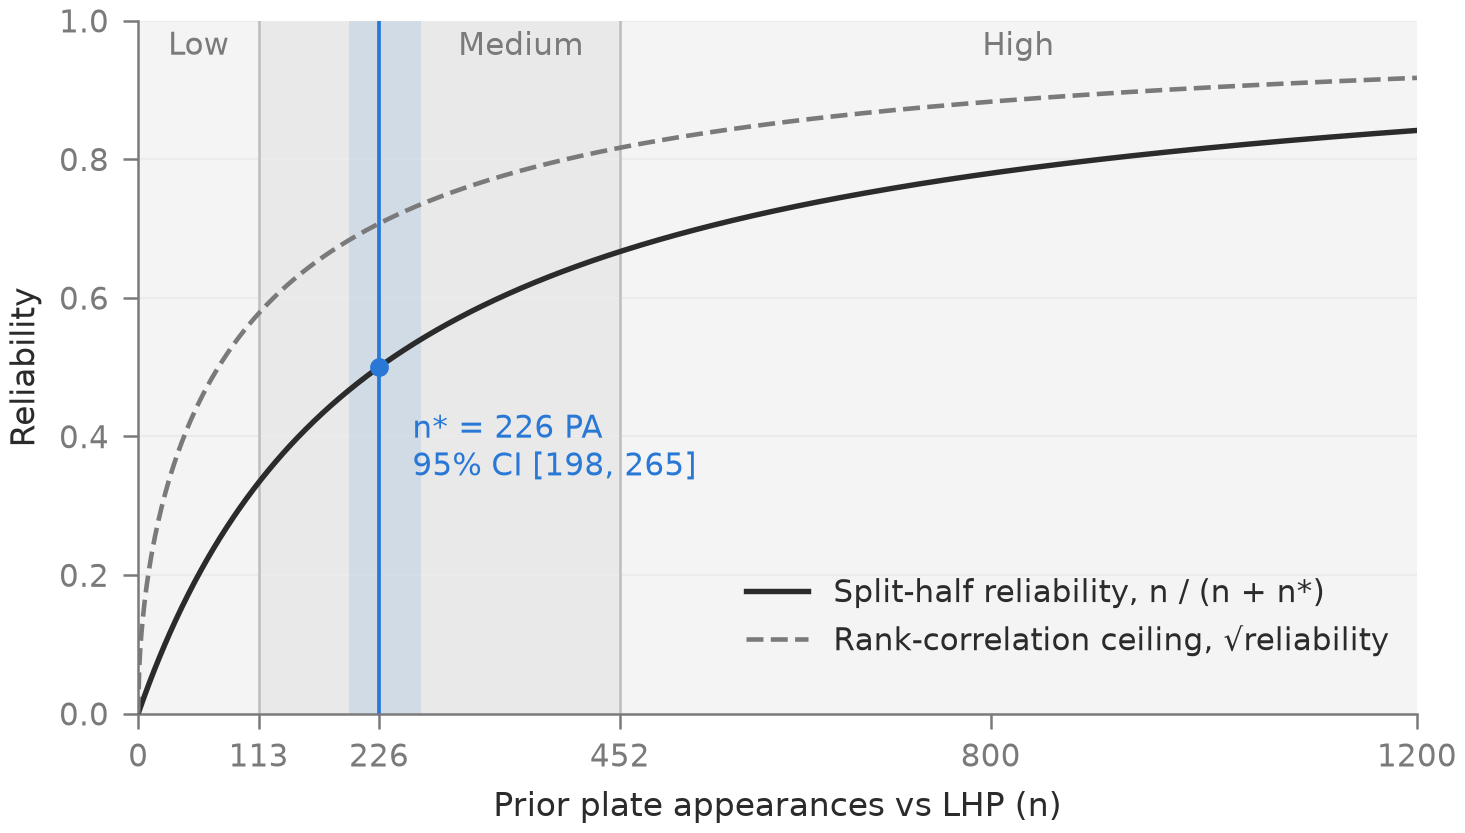
\includegraphics[width=0.62\linewidth]{fig_reliability.png}
\caption{\toreview Reliability of wOBA against left-handed pitchers by PA, training seasons, $n/(n+n^*)$, reaches 0.5 at $n^* = 226$ PA (shaded, 95\% interval 198 to 265). The vertical lines at 113 and 452 PA bound the low, medium, and high strata.}
\label{fig:reliability}
\end{figure}

% Source: src/analysis/baseline_ladder_bivariate_eb.py (3 trailing seasons, covariance by batter type);
% claim1_eval.py; paired CSV (2,000 batter-clustered draws); decision log 2026-07-30, 2026-09-20.
Two baselines are used. The empirical Bayes baseline takes a hitter's wOBA against each hand over the previous three seasons and shrinks the two sides jointly toward the league average for the hitter's batting side, with the correlation between sides estimated from the data. It generalizes the platoon regression of \citet{tango2007} by learning the amount of shrinkage. The boosted baseline is the gradient-boosted model described in Section~\ref{sec:intro}, fit on one row per hitter, season, and pitcher hand, using the same trailing outcomes plus the hitter's pitch summaries by pitcher hand and pitch group. The count enters it only as a two-strike indicator.

Each method is scored by root mean squared error (RMSE) and by Spearman rank correlation, both weighted by each unit's 2025 PA. Differences between the model and a baseline carry 95\% intervals from 2,000 bootstrap draws that resample batters. Before the 2025 model was trained, the low stratum was specified as the primary test. To pass it, the model had to beat the boosted baseline on RMSE and both baselines on rank correlation. All other comparisons are exploratory.\footnote{A version of the model with a 32-dimension embedding, trained with pitches to pitchers batting left in, was also scored on 2025. No comparison changed whether its interval excluded zero. Its low-stratum error differences nominally favored the baselines, while those of the final model nominally favor the model.}

% =====================================================================================
\section{Results}
\label{sec:results}

\subsection{How much signal one season holds}
\label{sec:ceiling}

% Source: results/measurement_ceiling_clean/differential_fraction_of_ceiling.csv (0.2965, 0.167);
% differential_exhibit.csv (0.1766, EB 0.1458, GBM 0.1413; RMSE 0.0633 vs floor 0.0639);
% level_ceiling_level_ceiling.json (0.742, 0.475); routes.json (fraction CI 0.264-0.910).
One season of outcomes limits how well any projection can score, so the size of that limit is measured before the projections are compared. Comparing the spread of hitters' observed values with the spread that sampling noise alone would produce gives the share of the spread that is real. This share is the same quantity as the reliability in Section~\ref{sec:eval}, and it sets the highest rank correlation any method could reach against those outcomes. The ceilings were computed on 2024, the selection season, for the 545 hitters with at least 10 PA against each hand. For a hitter's level, wOBA pooled over both hands, the ceiling is 0.742, and the model reaches 0.475, or 64\% of it (Figure~\ref{fig:ceiling}).

The platoon split is much harder to measure. True splits vary little across hitters compared with the noise in one season's observed split, so even a perfect projection would reach a rank correlation of only about 0.30 with it. After removing each batting side's average split, the model reaches 0.177, 60\% of that ceiling, compared with 49\% for empirical Bayes and 48\% for the boosted baseline. The model's share is imprecise (interval 26\% to 91\%, wide enough to hold both baselines' shares), and that interval holds the ceiling fixed, so the true uncertainty is larger. The share also depends on how the variance of true splits is estimated. That variance can instead be taken from 2024 alone, although small errors in the noise model can move this estimate by about its own size. With it, the ceiling falls to 0.167, below the model's 0.177. The share is a rough guide, not a measurement. The model's RMSE for the split is 0.0633, close to the 0.0639 floor that sampling noise sets, and empirical Bayes is about as close. One season of a hitter's observed split says little about whether any projection of that split was right.

% Source: paper/draft2/make_figs.py ceiling().
\begin{figure}[!ht]
\centering
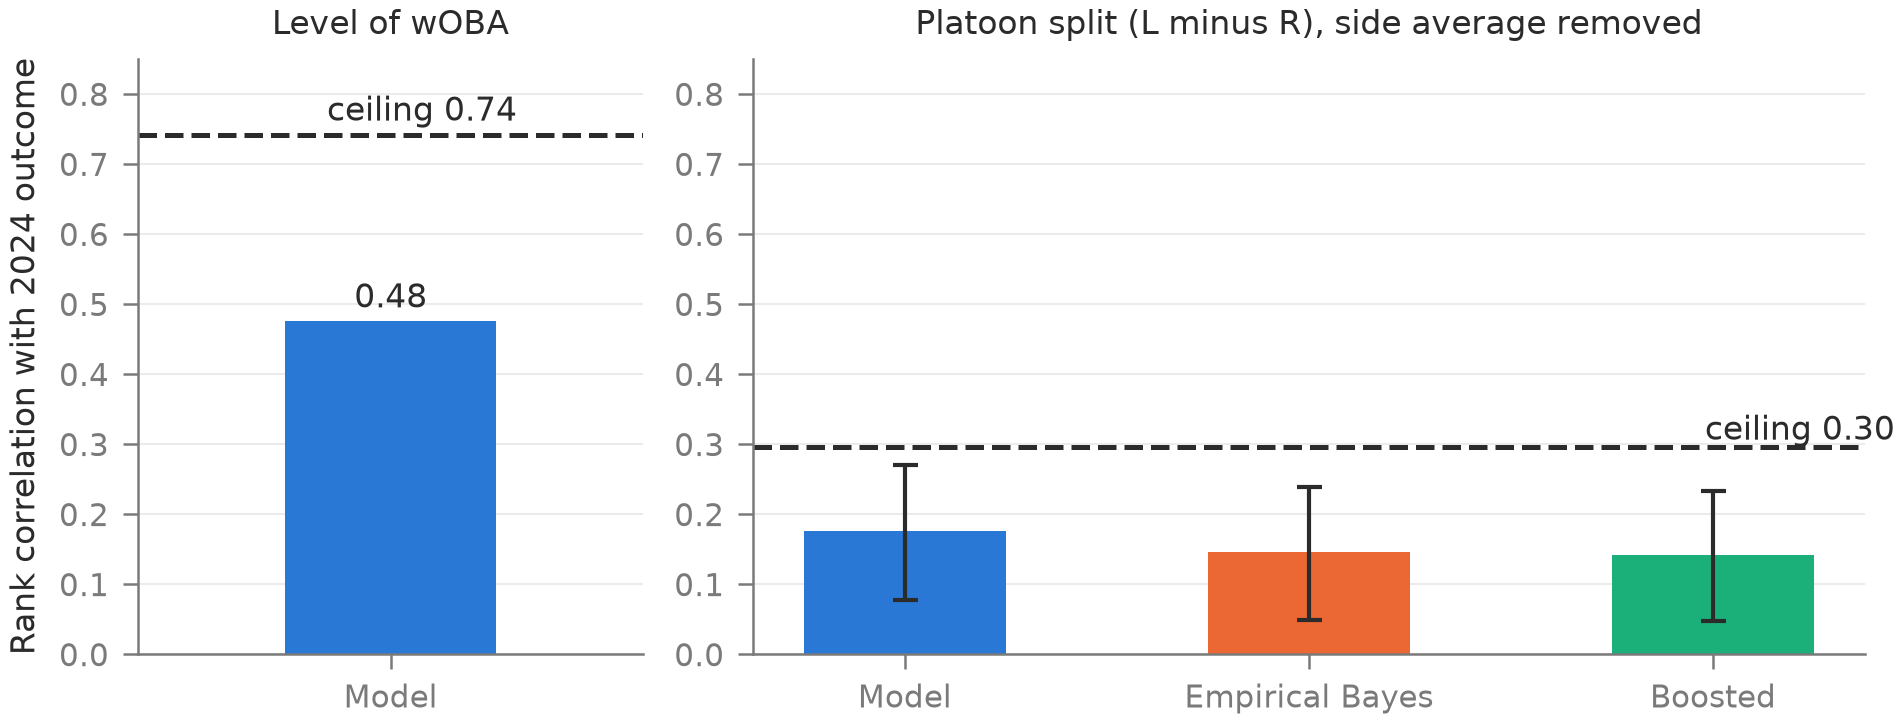
\includegraphics[width=0.85\linewidth]{fig_ceiling.png}
\caption{\toreview Rank correlation with 2024 outcomes against the ceiling one season allows, 545 hitters with at least 10 PA against each hand. Left, the level of wOBA pooled over both hands. Right, the platoon split after removing each batting side's average split, with 95\% intervals from resampling hitters. The dashed ceiling takes the variance of true splits from earlier seasons (0.296), and the dotted one from 2024 alone (0.167).}
\label{fig:ceiling}
\end{figure}

\subsection{Handedness splits on 2025}
\label{sec:test}

% Source: model_v1_claim1_scores_min_pa_sweep_clean_dim64_final.csv; paired CSV; verdict JSON.
The 2025 test scores each side's wOBA separately, a target that falls between the level and the split, with more real variation across hitters than the split and fewer PA behind each value than the level. The results by stratum and pooled can be seen in Table~\ref{tab:test}. Across all 1,157 units the model ties both baselines on error. Its RMSE is 0.0452 against 0.0453 for the boosted baseline and 0.0460 for empirical Bayes, and both difference intervals include zero. It orders hitters better than both, with a weighted rank correlation of 0.47 against 0.42 for the boosted baseline and 0.40 for empirical Bayes. The intervals on those two differences, 0.011 to 0.089 and 0.015 to 0.125, both exclude zero. Like every comparison outside the low stratum, these pooled comparisons are exploratory.

\begin{table}[!ht]
\centering\small
\begin{tabular}{lrrrrrrr}
\toprule
 & & \multicolumn{3}{c}{RMSE (lower better)} & \multicolumn{3}{c}{Rank corr. (higher better)} \\
\cmidrule(lr){3-5}\cmidrule(lr){6-8}
Prior PA & Splits & Model & GBM & EB & Model & GBM & EB \\
\midrule
Low & 384 & 0.0605 & 0.0609 & 0.0620 & 0.16 & 0.12 & 0.13 \\
Medium & 280 & 0.0455 & 0.0479 & 0.0492 & 0.42 & 0.28 & 0.22 \\
High & 493 & 0.0395 & 0.0385 & 0.0387 & 0.50 & 0.49 & 0.48 \\
All & 1157 & 0.0452 & 0.0453 & 0.0460 & 0.47 & 0.42 & 0.40 \\\bottomrule
\end{tabular}
\caption{Sealed 2025 side-specific wOBA. GBM: gradient-boosted; EB: empirical Bayes. Splits are hitter by pitcher hand. Medium is 113 to 451 prior PA.}
\label{tab:test}
\end{table}

The margin depends on prior exposure (Figure~\ref{fig:strata}). In the low stratum, the pre-registered test, the model's error is lower and its rank correlation higher than both baselines, but every interval spans zero, so the test was not passed. Of the stratum's 384 units, 164 (43\%) belong to hitters absent from the training data, and these share the generic projections of Section~\ref{sec:query}. The model cannot order these hitters among themselves, which leaves 220 of the 384 units where a hitter's own pitches inform the projection. The stratum holds 246 batters, and detecting the observed rank margin over the boosted baseline with 80\% power would take about 5,200.

The clearest signal is in the medium stratum, hitters with 113 to 451 prior PA against a hand. This comparison is exploratory. It is one of sixteen in Table~\ref{tab:test} (four rows, two baselines, two measures) and the only row where all four intervals exclude zero. There the model beats both baselines on both measures. Its rank correlation is 0.42 against 0.28 for the boosted baseline and 0.22 for empirical Bayes. Its RMSE is about 2 points of wOBA below the boosted baseline and 4 below empirical Bayes, against a typical error near 45 points. For these hitters the model's advantage lies mostly in ordering them. Among high-exposure hitters the three methods are even.

\begin{figure}[!ht]
\centering
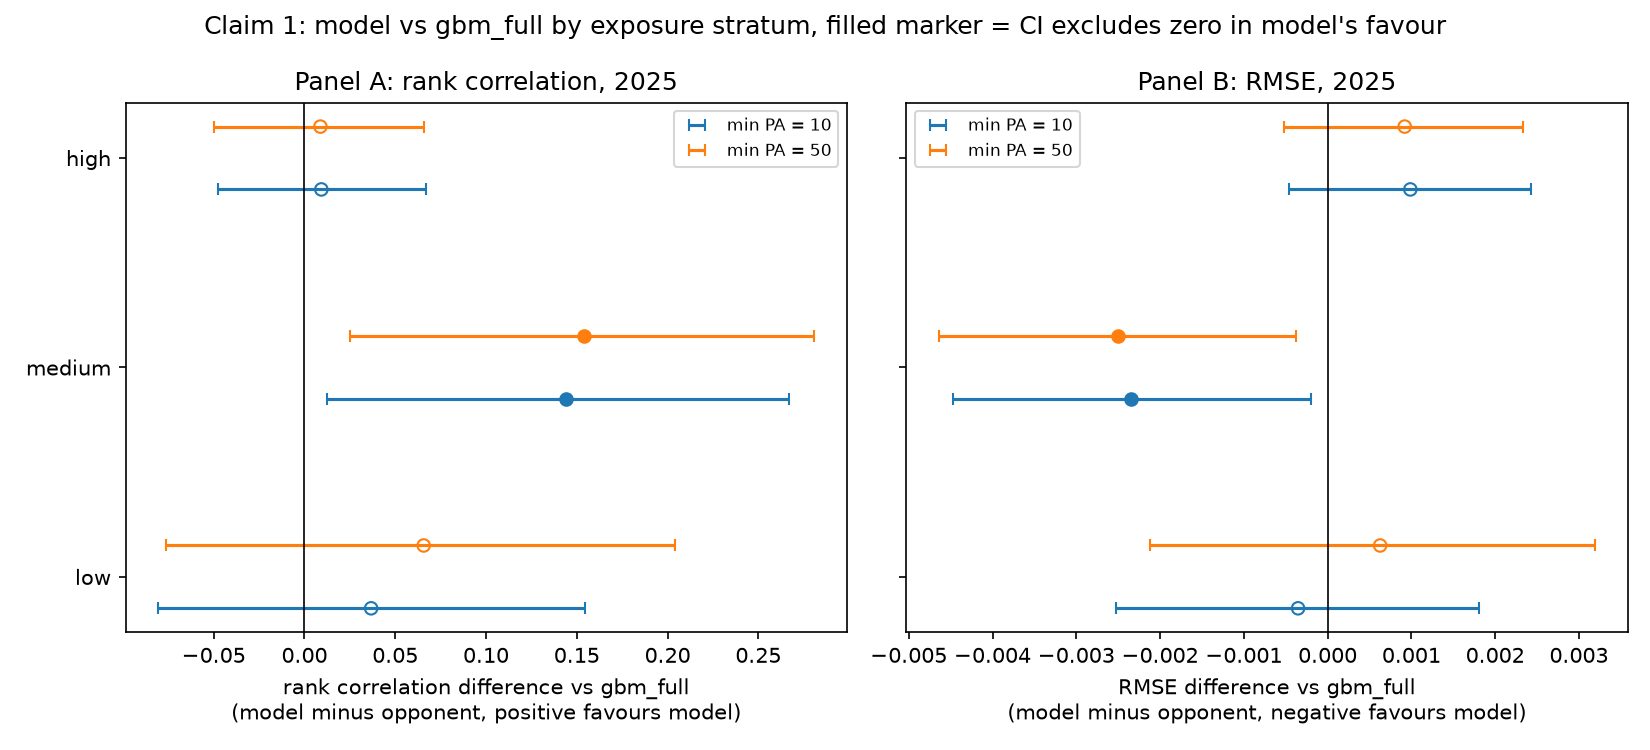
\includegraphics[width=0.72\linewidth]{fig_claim1_2025_strata.png}
\caption{\toreview The model's 2025 margin over the boosted baseline on error and on rank correlation, by prior-exposure stratum, at evaluation floors of 10 and 50 PA. Raising the floor from 10 to 25 or 50 PA changes no stratum's outcome, though at 50 PA the model's low-stratum RMSE is nominally above the boosted baseline's.}
\label{fig:strata}
\end{figure}

% Source: results/v_chain_clean/paper_figures/fig_calibration_2025 source JSON.
Calibration is poorest in the low stratum (Figure~\ref{fig:calibration}). A PA-weighted regression of each unit's observed 2025 wOBA on its projection gives a slope near one in the medium (0.98) and high (0.93) strata. There the projections are spread about as widely as the outcomes they predict. In the low stratum the slope is 0.59, so projections for little-seen hitters are spread more widely than their outcomes support. On average, a 10-point gap between two low-stratum projections corresponded to about 6 points of observed gap. Across all strata the slope is 0.81, below one by more than three standard errors. The projections are also off in level. High-stratum projections averaged about 9 points of wOBA above the observed values and low-stratum projections about 7 points below.

\begin{figure}[!ht]
\centering
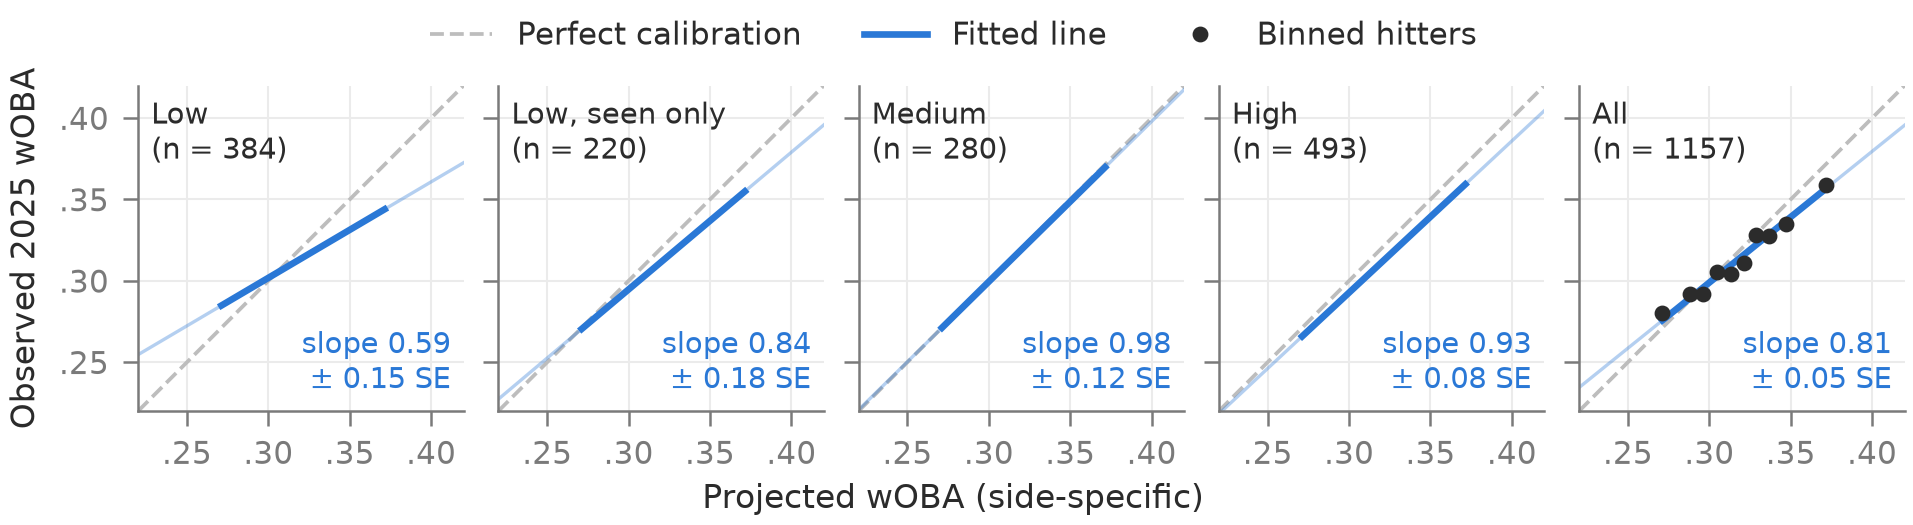
\includegraphics[width=0.95\linewidth]{fig_calibration_2025.png}
\caption{\toreview Calibration of 2025 side-specific projections by stratum. Each line is the PA-weighted regression of observed on projected wOBA. Points on the pooled panel are ten bins with equal PA. The dashed diagonal is perfect calibration.}
\label{fig:calibration}
\end{figure}

The model's prediction intervals are also too narrow. The intervals are built from the spread across the five seeds and each unit's sampling noise. Nearly all of the width comes from sampling noise. The seed spread alone gives a mean half-width of about 6 points of wOBA and covers 8\% of units, against about 105 points once sampling noise is added. On 2024, the nominal 95\% intervals covered the observed value for 87\% of 1,149 units. A band shown as 95\% would therefore miss about one unit in eight rather than one in twenty.

% Source: results/case_studies_2025/case_studies_2025.json (539, 296/243, wmae_model 0.0448 / wmae_eb 0.0462,
% within noise 519); all_hitters_bootstrap.json (diff 0.0014 [0.0002, 0.0026], share [0.506, 0.592]).
Because a platoon decision depends on the gap between a hitter's two sides, the model's projected split and the empirical Bayes split were also graded against each hitter's observed 2025 split. Across the 539 hitters with at least 10 PA against each hand in 2025, the model's projection was closer for 296 (55\%, interval 51\% to 59\%) and the empirical Bayes projection for 243. Weighted by the harmonic mean of each hitter's PA against the two hands, the model's mean absolute error is 0.0448 against 0.0462 for empirical Bayes. The difference, 0.0014 (interval 0.0002 to 0.0026), is about 1.4 points of wOBA. Both mean errors, near 45 points, are about as large as the largest projected split in Table~\ref{tab:cases}, which is consistent with the noise in one season's observed split described in Section~\ref{sec:ceiling}. The two projections got the direction of the observed split right about equally often, for 338 and 337 of the 539 hitters. For 519 of the 539 hitters, sampling noise in the observed split is large enough to reverse which projection is closer, so the comparison is informative only in aggregate.

Overall, the model did not pass the one pre-registered test. In exploratory comparisons it ties both baselines on error and orders hitters better than both, most clearly for hitters with a moderate track record. Its projected platoon splits are also slightly closer to the observed splits than those of empirical Bayes, though only in aggregate. For little-seen hitters its projections are spread too widely, and its prediction intervals are too narrow.

\subsection{Case studies and disagreements}
\label{sec:anchors}\label{sec:disagree}

% Source: docs/phase-v-spec.md V.8 (anchors and expectations written before results);
% results/case_studies_2025/case_studies_2025.{csv,json}.
The case studies are five well-known hitters, each with an expected platoon direction fixed before any projection was examined.\footnote{Alec Bohm replaced a pre-registered right-handed hitter whose training data showed no platoon split.} Joc Pederson and Kyle Schwarber are left-handed hitters with reputations as platoon hitters and should project worse against left-handed pitchers. Alec Bohm, a right-handed hitter, should project better against them. Mike Trout and Juan Soto play every day and should project close to flat. All five are high-exposure hitters, so they show how the model describes hitters it knows well. Each projected 2025 split can be seen in Table~\ref{tab:cases} beside the empirical Bayes projection and the observed split.

\begin{table}[!ht]
\centering\small
\begin{tabular}{llrrrr}
\toprule
Hitter & Bats & Model & EB & Observed (SE) & $z$ \\
\midrule
Joc Pederson & L & $-0.047$ & $-0.039$ & $+0.172$ (0.121) & 1.77 \\
Kyle Schwarber & L & $-0.042$ & $-0.028$ & $+0.025$ (0.039) & 1.52 \\
Juan Soto & L & $-0.041$ & $-0.044$ & $-0.074$ (0.041) & 0.78 \\
Mike Trout & R & $+0.009$ & $+0.007$ & $-0.062$ (0.056) & 1.25 \\
Alec Bohm & R & $+0.022$ & $+0.033$ & $+0.042$ (0.052) & 0.28 \\
\midrule
Aaron Judge & R & $+0.020$ & $+0.003$ & $+0.038$ (0.049) & 0.54 \\
José Altuve & R & $+0.021$ & $+0.026$ & $+0.013$ (0.051) & 0.22 \\
Marcell Ozuna & R & $+0.020$ & $+0.002$ & $-0.006$ (0.050) & 0.33 \\
\bottomrule
\end{tabular}
\caption{2025 platoon split (wOBA against left-handed pitchers minus wOBA against right-handed pitchers) for the five case-study hitters (top) and three high-exposure hitters among the twenty on whom the model and empirical Bayes disagreed most in 2024 (bottom). SE is the standard error of the observed split, and $z$ is the distance of the observed split from the midpoint of the two projections in standard errors.}
\label{tab:cases}
\end{table}

The projections match four of the five expectations. Pederson and Schwarber project worse against left-handed pitchers, Bohm better, and Trout close to flat. Soto, expected to be flat, projects 0.041 worse against left-handed pitchers, and Soto's observed 2025 split of $-0.074$ runs the same way. Empirical Bayes matches the same four expectations and also projects Soto worse against left-handed pitchers ($-0.044$), so the case studies do not separate the two methods on direction. Empirical Bayes was closer for all five in 2025, by 0.002 to 0.014. Every $z$ in Table~\ref{tab:cases} is below 1.96, however, which means noise alone could reverse which projection is closer. Pederson shows the size of that noise. With 19 PA against left-handed pitchers in 2025, Pederson's observed split of $+0.172$ has a standard error of 0.121, wide enough to hold either projection and the opposite sign.

% Source: results/v_chain_clean/disagreement_summary.json, disagreement_top.csv;
% case_studies_2025.csv (disagreement rows, stratum by 2025 prior PA).
% Disagreement rank scatter (fig_disagreement.png) dropped from the text.
Hitters on whom the model and empirical Bayes disagree show where pitch-level information moves a projection away from a hitter's outcome history. The 2024 projections compared here come from the first seed of the selection model, trained through 2023. Across 545 hitters in 2024, the two methods' projected splits have a Spearman correlation of 0.77. The correlation is 0.80 and 0.79 in the low and medium strata and 0.69 in the high stratum. Lower agreement in the high stratum is consistent with empirical Bayes shrinking least for hitters with long outcome histories, while the model's projection still rests on how the hitter handles each pitch.

With hitters ranked within batting side, the largest disagreement is Robbie Grossman, first among right-handed hitters by empirical Bayes and 324th by the model. Marcell Ozuna is the reverse, 6th by the model and 316th by empirical Bayes, and Aaron Judge and José Altuve also rank much higher by the model. Ozuna, Judge, and Altuve are graded against 2025 in Figure~\ref{fig:cases}, along with six medium-stratum hitters from the twenty largest disagreements. Most of these observed splits have a standard error between 0.04 and 0.06, and a few have one near 0.1. These errors are at least the size of the gaps being graded, so the cases show how the two methods differ rather than which is right. The evidence on split accuracy remains the 539-hitter comparison in Section~\ref{sec:test}.

% Source: paper/draft2/make_figs.py cases().
\begin{figure}[!ht]
\centering
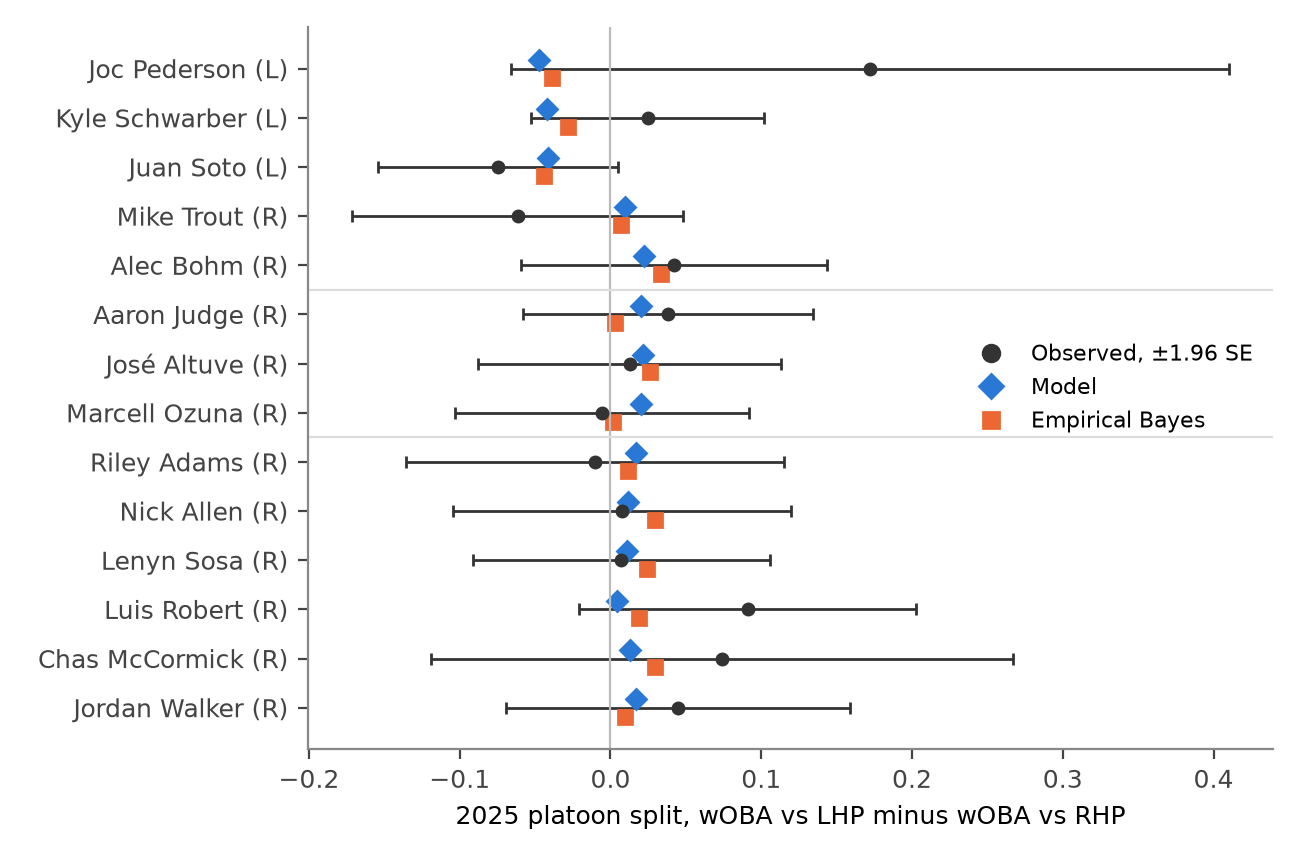
\includegraphics[width=0.78\linewidth]{fig_cases.png}
\caption{\toreview 2025 platoon splits for the five case-study hitters (top), the three high-exposure disagreements in Table~\ref{tab:cases} (middle), and the six medium-stratum hitters among the twenty largest 2024 disagreements (bottom). Each observed split has a 1.96 standard error bar beside the model and empirical Bayes projections.}
\label{fig:cases}
\end{figure}

\subsection{What the embedding learned}
\label{sec:embedding}

% Source: results/v_chain_clean/embedding_structure/embedding_structure.json (norm r 0.934, PC1 r
% 0.090, silhouette max 0.054, neighbour purity); embedding_alt_views.json (LDA 5-fold, n 1,493,
% power 0.791, contact 0.754, zone swing 0.746, chase 0.734); seed_stability_corrected_null.json
% (0.837 vs 0.123). Selection model (trained through 2023).
The loss scores single pitches and never sees a hitter-level statistic such as a contact rate or a 90th-percentile exit velocity, so any such summary present in the embedding was assembled by the model. The analyses in this section and those that follow use the selection model, trained through 2023. The head outputs, the response surfaces, and the named nearest neighbors come from its first seed alone. For the classifiers here and the neighborhood summaries in Section~\ref{sec:neighbors}, each hitter's embedding is averaged over the five seeds and scaled to unit length.\footnote{The five seeds give similar vectors for the same hitter, with a median cosine similarity of 0.83 after rotating each onto the first, against 0.12 when hitters are shuffled before the rotation is fit. Embeddings are averaged after this alignment. They are scaled to unit length because an embedding's length grows with the hitter's exposure (correlation 0.93 with log prior PA), and after scaling the main direction of variation is nearly unrelated to playing time (0.09).} Hitters were split into thirds on attributes measured from their own pitches, and a linear classifier on the embedding was fit to recover each hitter's third under five-fold cross-validation. Across 1,493 hitters it recovers the power third (90th-percentile exit velocity) for 79\% of hitters and the contact third (contact rate on swings) for 75\%, against 33\% by chance. In-zone swing rate (75\%) and chase rate (73\%) are recovered nearly as well. Each hitter can be placed on the fitted power and contact directions (Figure~\ref{fig:powercontact}), and mean observed wOBA rises toward high power and high contact. Positions on the two fitted directions correlate at $-0.44$, against $-0.22$ for the observed statistics, so the figure overstates how much power and contact trade off across hitters. This indicates that the embedding organizes hitters by power and contact, although the model was never given either statistic.

\begin{figure}[!ht]
\centering
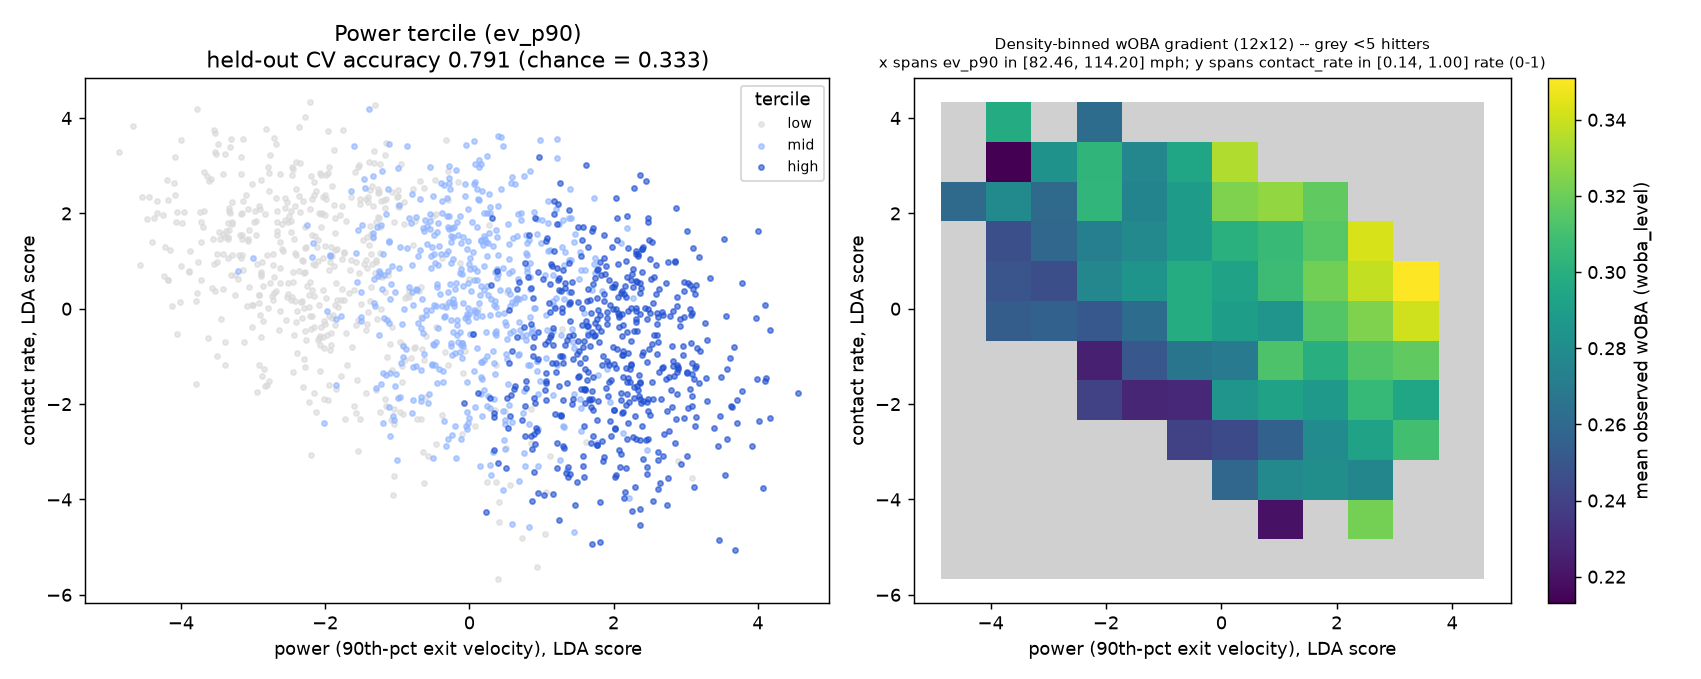
\includegraphics[width=0.95\linewidth]{fig1_power_contact.png}
\caption{Hitters placed by the embedding on fitted power and contact directions. Left: observed power tercile. Right: mean observed wOBA per cell.}
\label{fig:powercontact}
\end{figure}

% Source: make_figs3.py fig_miss_damage (asserts match to v_chain_clean/embedding_structure/
% embedding_alt_views.json); decision log (spin vs fastball pairings).
The embedding separates some skills by pitch type and not others. For each of two skills, two directions were fit in the embedding, one for breaking balls and one for fastballs (Figure~\ref{fig:missdamage}). For whiff rate the two directions correlate at 0.64 across hitters, and many hitters sit well off the diagonal. Relative to other hitters, they rank much worse against one pitch family than against the other. Their observed whiff rates on the two families correlate at 0.53. For power, measured by 90th-percentile exit velocity, the two directions correlate at 0.94 and the observed values at 0.83. Both correlations in the embedding run about 0.11 higher than the observed ones, partly because the two directions share the embedding's main direction of variation. The embedding follows the data on both skills. Whiff rate differs by pitch family in the observed values and in the embedding, and power is close to a single skill in both.

\begin{figure}[!ht]
\centering
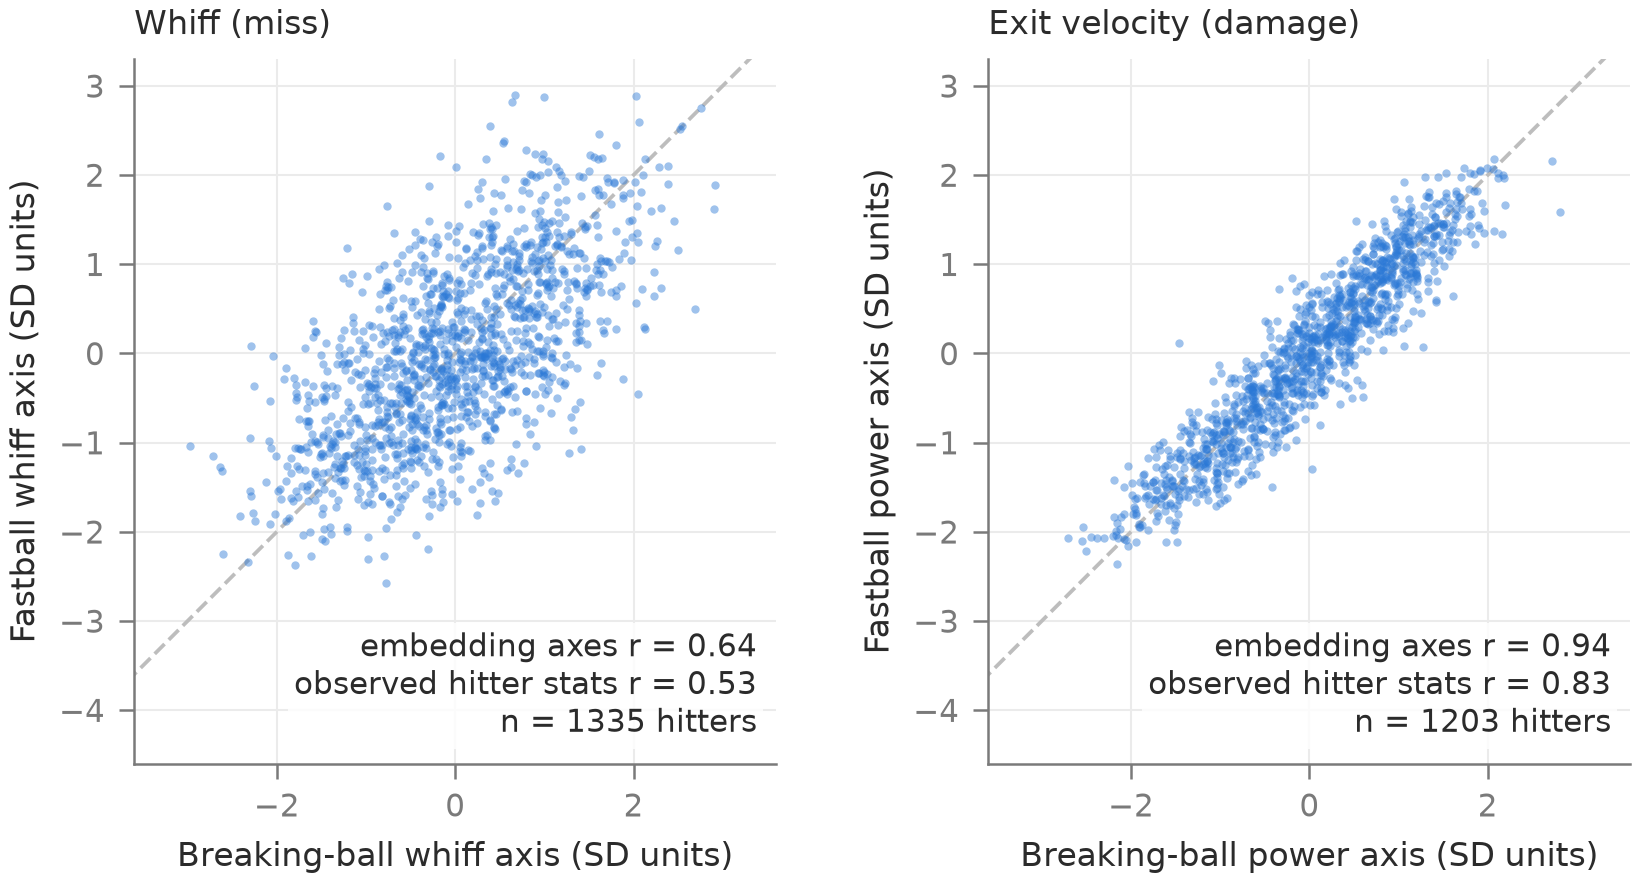
\includegraphics[width=0.8\linewidth]{fig_miss_damage.png}
\caption{\toreview Each hitter placed on embedding directions fit to breaking-ball and fastball whiff rate (left, 1,335 hitters) and to breaking-ball and fastball power, 90th-percentile exit velocity (right, 1,203 hitters), in standard deviations. The dashed line is equal standing on both pitch families.}
\label{fig:missdamage}
\end{figure}

% Source: results/v_chain_clean/fig_head_partial_heatmap source (to confirm in figs3_report.md).
Each head draws on the embedding for a different part of the plate appearance. A head's hitter-specific output is its average prediction for the hitter over a fixed set of 2,000 training-season pitches. Figure~\ref{fig:headpartial} correlates this output with the hitter's observed training-season statistics after removing log prior PA. The swing head tracks swing rate (0.67), the contact head tracks whiff rate ($-0.56$), the exit velocity head tracks bat speed (0.61, for the 570 hitters with bat tracking), and the launch angle and spray heads track average launch angle (0.49) and pull rate (0.34). In each case the head's output follows the standard statistic for its own part of the plate appearance.

\begin{figure}[!ht]
\centering
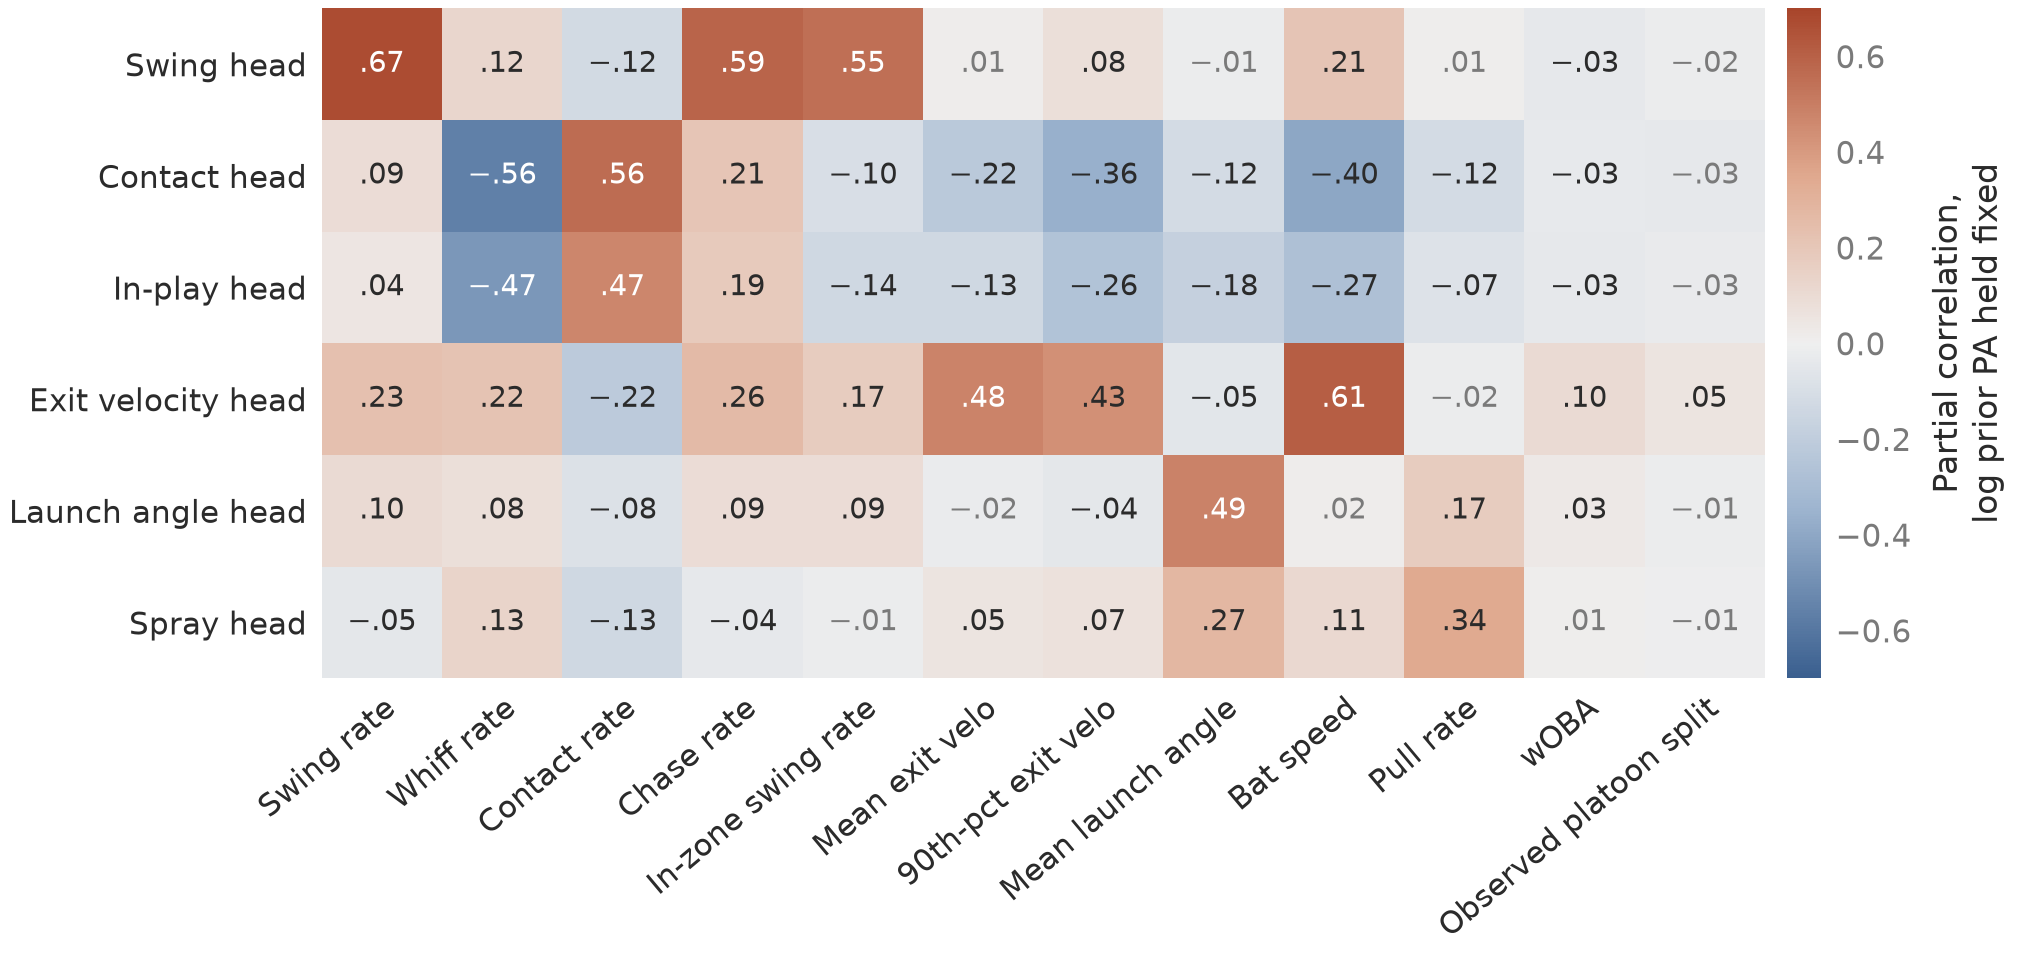
\includegraphics[width=0.78\linewidth]{fig_head_partial.png}
\caption{\toreview Correlation between each head's hitter-specific output and observed hitter statistics, training seasons, after removing log prior PA.}
\label{fig:headpartial}
\end{figure}

% Source: embedding_structure/neighbour_purity.csv; paper_figures/platoon_sign_agreement.json
% (310/545, null 0.498); platoon/platoon_projection.json (cosine 0.142 [0.081, 0.201], partial r
% 0.074 / 0.144 / 0.133). Platoon-direction bar figure (fig_platoon_direction.png) dropped from the text.
The embedding also holds the platoon split, but more weakly than power or contact. No head's output tracks a hitter's observed platoon split closely (Figure~\ref{fig:headpartial}). Every correlation is 0.05 or below in size, and only the exit velocity head's interval excludes zero. After removing each batting side's average split, the model's projected 2024 split has the same sign as the observed split for 310 of 545 hitters (57\%), against 50\% when hitters are shuffled. Perturbing each embedding dimension gives the direction along which the projected left-minus-right gap grows. This direction has a cosine of 0.14 (interval 0.08 to 0.20) with a separate direction fit to decode the empirical Bayes split, so the two are related but far from the same. A hitter's position along the model's direction correlates with the observed split in the training seasons, after removing log prior PA, at 0.07 in the low stratum, 0.14 in the medium, and 0.13 in the high, each with an interval above zero. The split is a faint direction in the embedding, and it is faintest in the low stratum, where the pre-registered 2025 test was not passed.

\subsection{What the model sees in a hitter}
\label{sec:sees}

% Source: results/v_chain_clean/surfaces_location.csv (quantity q, delta x1000; selection model
% clean_clean_dim64); make_figs3.py fig_surfaces; case_studies_2025.json (Pederson head outputs).
Because the network scores single pitches, it can be read one pitch location at a time. Figure~\ref{fig:surfaces} shows, for each case-study hitter, the expected wOBA on a ball in play by location, relative to the average of 100 hitters on the same pitches. Schwarber and Soto hit best on pitches in the upper middle of the zone, up to about 170 points above average, and Soto falls below average on low pitches. Trout's best results come on low pitches over the middle, at about 200 to 220 points above average. Bohm's surface is nearly flat. It averages about 30 to 40 points above the average hitter, with no cell above about 70.

Each hitter's surface also changes little between pitcher hands. On contact, Pederson averages 44 points above the average hitter against left-handed pitchers and 48 against right-handed pitchers. The swing head shows a larger difference. Pederson swings less often than an average hitter against both hands, by about 2.2 percentage points against left-handed pitchers and 1.2 against right-handed pitchers, while making contact slightly more often than average against both. These differences are small and on different scales, so they do not say which part of the plate appearance produces the projected gap. Because each head covers one part of the plate appearance, the heads can point to where a projected split may come from, which a projection built only from outcomes, such as empirical Bayes, cannot.

\begin{figure}[!ht]
\centering
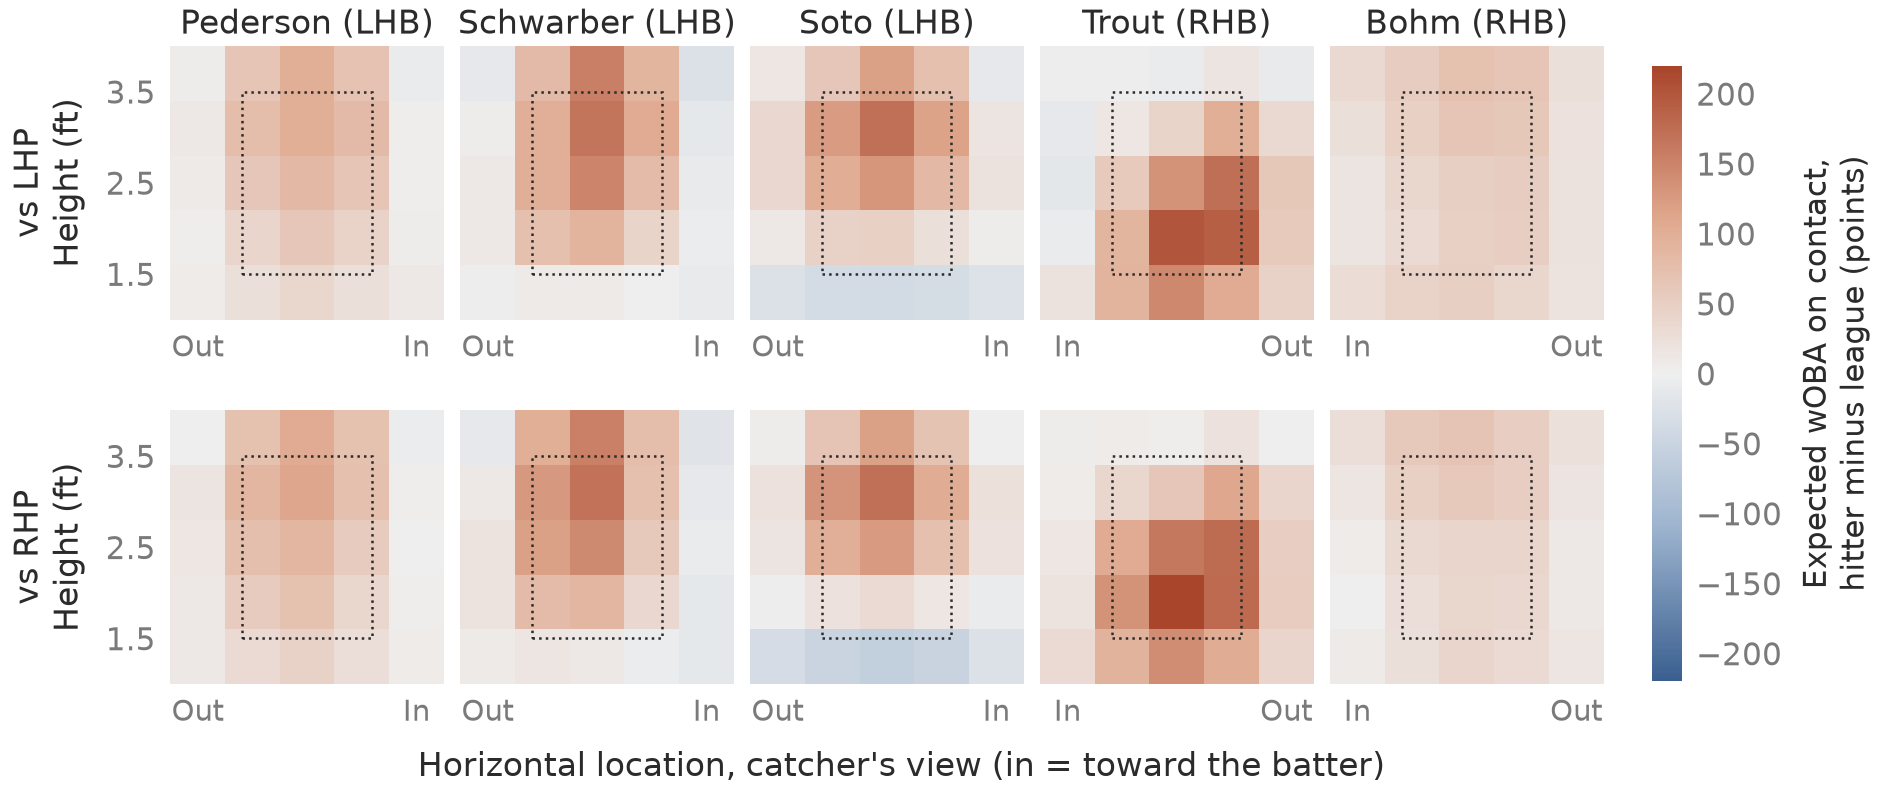
\includegraphics[width=\linewidth]{fig_surfaces.png}
\caption{\toreview Expected wOBA on a ball in play by pitch location, hitter minus the average of 100 hitters on the same 2015 to 2023 pitches, in wOBA points, against left-handed (top) and right-handed (bottom) pitchers. Red is above the average hitter and blue below. Locations are from the catcher's view, with ``in'' toward the batter. The dotted box is the strike zone.}
\label{fig:surfaces}
\end{figure}

\subsection{Nearest neighbors}
\label{sec:neighbors}

% Source: results/v_chain_clean/neighbours_high.csv; embedding_structure.json (silhouette max 0.054,
% k 2 to 10); embedding_structure/neighbour_purity.csv (0.57 vs 0.33).
Nearest neighbors in the embedding show what the model treats as similar. The named lists below use the first seed's embedding, scaled to unit length, and averaging over the five seeds changes several of the names, so the lists illustrate the space rather than define it. Among high-exposure hitters, Pederson's eight nearest neighbors are Kyle Schwarber, Joey Gallo, Justin Smoak, Harrison Bader, Logan Morrison, Franmil Reyes, Ryan Zimmerman, and Matt Chapman, mostly power hitters from both sides of the plate. Trout's are Ronald Acuña, Pete Alonso, Brandon Belt, Eugenio Suárez, Austin Jackson, Anthony Rendon, Howie Kendrick, and Christian Walker. When hitters are instead ranked by ten observed statistics covering plate discipline, contact quality, and wOBA, Trout's eight nearest include Yordan Álvarez, Paul Goldschmidt, Juan Soto, and Mookie Betts, and only Ronald Acuña appears on both lists. Across the five case-study hitters the two kinds of list share 9 of 40 names, which suggests that the embedding's notion of similarity differs from one built on season statistics.

Hitters within a neighborhood are similar in skill, but the neighborhoods do not form separate groups. A hitter's ten nearest neighbors share the hitter's power third 57\% of the time, against 33\% with shuffled labels. The silhouette score is near zero when groups overlap, and here it is at most 0.054 for any number of clusters from two to ten. The space holds neighborhoods of similar hitters, not a set of hitter types.

\subsection{Other queries}
\label{sec:otherqueries}

% Source: results/v_chain_clean/paper_figures/level_query_heldout.json (partial on log prior PA,
% held-out 2024, min 10 PA); results/pitcher_type_query_clean/ceiling.csv (split-half reliability).
% Level-query figure (fig_level_query.png) dropped from the text.
Any set of pitchers defines a query, and only the handedness query was tested against baselines. Two others show what the approach supports and how far one season of outcomes can check it. The level query averages a hitter's two handedness projections from Equation~\eqref{eq:query} and is the pooled projection whose ceiling share appears in Section~\ref{sec:ceiling}. After removing log prior PA, its correlation with wOBA in the 2024 selection season is 0.38 across 521 hitters (interval 0.30 to 0.45). The correlation rises with exposure, from 0.17 in the low stratum to 0.38 in the medium and 0.52 in the high. This suggests that the level query carries information about a hitter's 2024 wOBA beyond how much the hitter had played.

A query over pitcher traits, such as right-handed pitchers in the top third of fastball velocity, is computed the same way but is harder to check. Checking it needs an observed contrast, such as a hitter's wOBA against the top third of right-handed pitchers by fastball velocity minus the wOBA against the bottom third. Across 301 hitters in 2024 this contrast has a split-half reliability of 0.08 (interval $-0.15$ to 0.26), and the same right-handed contrasts for fastball height and breaking-ball share are no higher. One season of outcomes cannot separate these matchup effects from noise, so the model's projections for them remain untested.

% =====================================================================================
\section{Discussion}
\label{sec:discussion}\label{sec:ordering}

% Source: Section 3 numbers.
The model is better at saying which of two hitters will do better against a hand than at saying by how many points. Part of this is a property of the data. Empirical Bayes sits just as close to the error floor for the split (Section~\ref{sec:ceiling}), so one season of outcomes cannot show much skill at sizing a split for any method. The model's intervals are also too narrow to size one reliably. Many lineup decisions depend on order rather than size. Choosing which of two bench hitters starts against a left-handed pitcher, the decision described in Section~\ref{sec:intro}, is a ranking question, and a few points of error in both projections do not change the call if the two are in the right order.

The model's advantage over the baselines varies with exposure, and because the strata cuts are a convention, the pattern is better read as a curve than as three groups. With heavy exposure, several seasons of outcomes already measure a hitter well, which leaves little for any method to add. With moderate exposure, a hitter has seen enough pitches from a hand for the embedding to describe how the hitter handles them, while the outcomes of those plate appearances are still too few to stabilize. Pitch-level outcomes accumulate several times faster than plate appearance results (Section~\ref{sec:intro}). This would explain why the clearest gain appears in this range, although that gain was found in exploratory analysis. With little exposure, the model's point estimates still order hitters better than both baselines do, but every interval spans zero and the projections are spread more widely than the outcomes support (calibration slope 0.59). For a team, the model is most useful for ranking platoon options among hitters with a moderate track record, where the decision is still in question. It is not a replacement for a projection system on raw accuracy.

% =====================================================================================
\section{Future directions}
\label{sec:future}

% Source: docs/decision-log.md (2026 medium-band registration; power ~60% of batters needed);
% measurement_ceiling_summary.json (coverage 0.8695).
The model turns per-pitch hitter outcomes into a projected wOBA against any chosen set of pitchers. The most direct application is a matchup card that ranks a team's options against a pitcher hand, the query tested here, and shows a band around each projection. Other weightings would serve other decisions, though they are untested here. A team preparing for a series could weight the opposing staff by the innings each pitcher is expected to throw, and a team choosing a pinch hitter could set $S$ to the single reliever warming up. The same approach could support roster questions. A candidate hitter's projections against the pitchers a team expects to face can be set beside those of the hitters already on the roster. This is a single-split version of the counterfactual roster comparison that \citet{alcorn2018} proposed for player embeddings.

Three steps stand between the model and those uses. The prediction intervals are too narrow and need recalibration before a card can show a band. The moderate-exposure advantage was found in exploratory analysis and is registered as a secondary hypothesis for 2026. Detecting it at its 2025 size with 80\% power would take about 377 batters, against 236 in the 2025 medium stratum, so 2026 may need to be pooled with later seasons. The measurement ceiling should also be recomputed on a season not used for model selection. The low-exposure margin is a separate question. It is nominally positive but underpowered, and confirming it at its observed size would take about 5,200 batters, roughly 21 times the 246 in the stratum.

Other extensions would widen what the model can answer. The velocity, location, and single-pitcher queries need held-out targets and baselines of their own before they can inform decisions. Hitters absent from training now receive one of four generic projections and need a better starting point. One option is a prior built from what is known about them. Another is minor league data mapped into the same space, as \citet{alcorn2018} suggested. Finally, the count is the only game state the model sees, and the score, inning, and runners could be added.

\bibliographystyle{plainnat}
\bibliography{refs}

\end{document}
